\begin{figure}[h!]
    \centering
    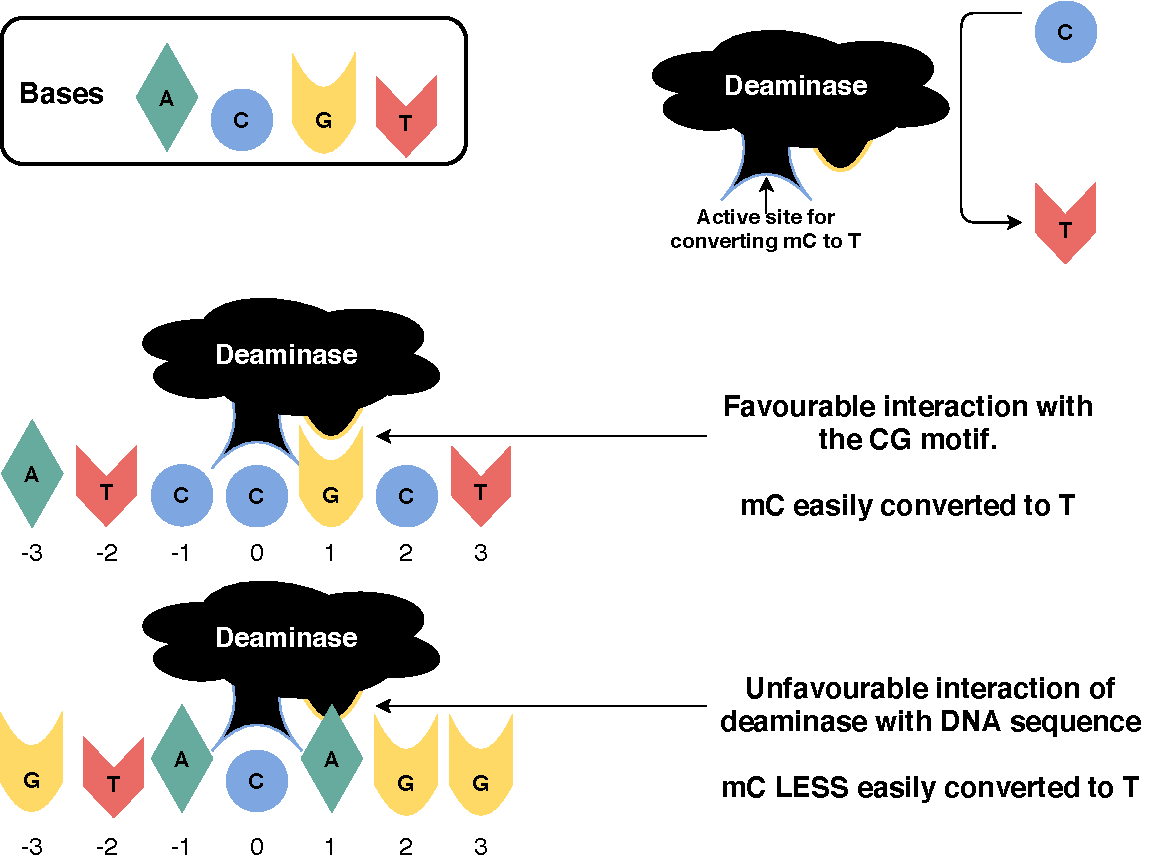
\includegraphics[scale=0.78]{graphics/motif_demo.pdf}
    \caption{\textbf{Methyltransferase activity as an example to explain how mutations are closely linked with the bases next to them}. Methyltransferase favours the CG motif, so CG is easily methylated into mCG. mC is an ``excited'' state that is prone to C$\rightarrow$T mutations. While many publications focus on the 3-mer context of mutations (pos -1, 0 and 1), which includes the base change and two bases immediately next to it, evidence shows that bases outside the 3-mer could also be influential. This project seeks to explore the information content available in larger sequence contexts than 3-mers.}
    \label{fig:motif_demo}
\end{figure}
